\documentclass{article}
\usepackage[utf8]{inputenc}
\usepackage{fancyhdr}
\usepackage{lipsum}
\usepackage{graphicx}
\usepackage{ulem}
\usepackage{wrapfig}
\newpage{}
\begin{document}
	\pagestyle{fancy}
	\fancyhead{}
	\fancyhead[RO,LE]{\textbf{Broj $e$ i primene u finansijama}}
	\section*{\uline{Primena broja e u finansijama}}
	\begin{wrapfigure}{r}{0.5\textwidth}
		\begin{center}
			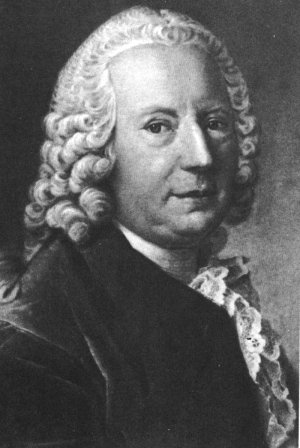
\includegraphics[width=0.33\textwidth]{bernuli.jpg}
		\end{center}
		\caption{Danijel Bernuli}
	\end{wrapfigure}
	\paragraph{\normalfont{Vrednost broja e u početku je računata u bankarse svrhe.
			Kao što je rečeno, smatra se da je problem broja e bio vezan za finansije. Danijel Bernuli ispitivao je kamatnu stopu i različite dohotke na osnovu učestalosti ulaganja.}}
	\section*{\uline{O Bernuliju}}
	Sticao je znanja iz matematike i prirodnih nauka, predavao je matematiku, anatomiju, botaniku i fiziku. Bio je prijatelj Leonarda Ojlera, zajedno su saradjivali na više polja matematike i fizike. Različiti problemi koje je pokušavao da razreši (teorija elastičnosti, mehanika talasa) nagnali su ga da razvije takav matematički aparat kao što su diferencijlne jednačine i redovi.
	\section*{\uline{Značaj u finansijama}}
	Pretpostavimo da u banku ulažemo sumu novca h. Ako bi banka davala 100%-tnu kamatu,
	za godinu dana mogli bismo da podignemo sumu novca 2h. Ukoliko bismo posle pola
	godine podigli novac i opet ga uložili nakon godinu dana suma novca iznosila bi
	\begin{equation} (1+\frac{1}{2})^2*x. \end{equation}
	Ako bi smo ovaj postupak primenjivali svaki dan, nakon godinu dana suma novca
	iznosila bi $((1+\frac{1}{365})^3^6^5*x)$. Sad, postavlja se pitanje koliko novca bi mogli da zaradimo kada bi banka računala složen interes n beskrajno malim vremenskim intervalima tzv. „neprekidno kapitalisanje“? Odgovor je:
	\begin{equation} \lim_{n \rightarrow \infty} (1+\frac{1}{n})^n=e \end{equation}
	\newpage{}
	\section*{\uline {Zakljčak}}
	\paragraph{\normalfont{U cilju približavanja teme čitaocu i lakšeg razumevanja, ovaj rad izrađen je kroz teorijska objašnjenja i praktične primere čija je tačnost potvrđena. Fokus ovog rada bio je na jednoj konstanti čija se važnost i primena ne ogledaju samo na polju matematike već i u svakodnevnom životu. Iako mi toga možda nismo svesni, ovo otkriće u matematici doprinelo je razvoju mnogih drugih sfera kao što su biologija, fizika, hemija, bankarstvo, računovodstvo... Pošto se broj e kao zasebna tema ne izučava toliko u školi već se spominje kroz druge pojave, nadam se da sam kroz ovaj rad uspela da objasnim značaj i istorijski razvitak ovog broja.}}
	
	\section*{\uline {Literatura}}
	\paragraph{\normalfont
		{1. Vene T. Bogosavov, Zbirka rešenih zadataka iz matematike 3, za 3. razred srednje škole, Zavod za udzbenike i nastavna sredstva, Beograd, 2013.\\
			2. S. Ognjanović, Ž. Ivanović, Krugova zbirka zadataka i testova iz matematike za 3. razred gimnazija i tehničkih škola, Krug, Beograd, 2010.\\
			3.\url{ http://elementarium.cpn.rs/teme/sedam-najlepsih-brojeva/} \\
			4.\url{https://www.matematika.edu.rs/saznajte-zanimljivosti-o-broju-e/}\\
			5.\url{https://www.iserbia.rs/da-li-ste-znali/dan-broja-pi-broj-e-314-271/}\\
			6.\url{http://poincare.matf.bg.ac.rs/}\\
			7.\url{http://alas.matf.bg.ac.rs/~mn06070/Broj_e.pdf/}}}\\
\end{document}